\documentclass[11pt]{article}
\usepackage{graphicx}
\usepackage{hyperref}
\usepackage{natbib}
\usepackage{indentfirst}
\usepackage{subcaption}




\setlength{\textwidth}{6.5in}
\setlength{\headheight}{0in}
\setlength{\textheight}{8.0in}
\setlength{\hoffset}{0in}
\setlength{\voffset}{0in}
\setlength{\oddsidemargin}{0in}
\setlength{\evensidemargin}{0in}
\title{Predicting Mean Free Path of near surface quantum wells from AFM morphology using Contrastive Learning}
  
\author{Krishna N. Dindial }


\begin{document}


\maketitle

\section{Abstract}

III–V quantum well heterostructures are a platform for realizing hybrid superconductor–semiconductor devices, where electron mean free path in the quantum well is a key performance metric.
These thin film heterostructures are grown with slight lattice mismatch and as a result, develop a crosshatch surface pattern due to strain relaxation and the formation of misfit dislocations.
The crosshatch pattern likely contains information about the defects and the strain in the near surface well, and therefore could provide information about the mean free path of electrons confined to the well.
Prior work by Strohbeen et al. approached this problem by first extracting engineered features from AFM data such as characteristic wavelength and amplitude of the crosshatch pattern along orthogonal directions \cite{strohbeen2024}. These features were then fed to a machine learning algorithm to predict dislocation density paramaters in a physical model, which in turn were used to predict mean free path. 
While this seems 
useful and interpretiable for a physicist or material scientist, this pipeline relies on preprocessing steps and is not in the true spirit of machine learning.

\par
Instead I will investigate an approach to directly map AFM topography to mean free path without explicit feature extraction or intermediate modeling. I will train 
a supervised nueral network on raw AFM images. In addition I will suppliment the training and test sets with rotated afm images to reduce sensitivity to arbitraty scan orientiation. This way the model can learn morphology-transport relationships directly from data without being sensitive to the orientation of the sample when it was loaded into the afm.
I will find out if it is possible to predict the mean free path without manual alignment of afm images or handcrafted features.
\begin{figure}
    \centering
    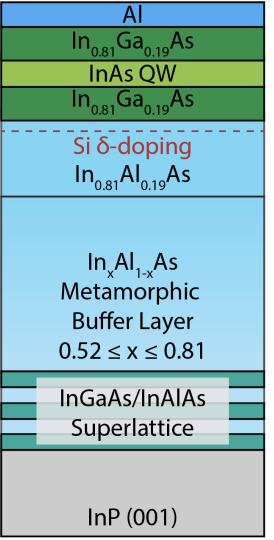
\includegraphics[width=0.3\textwidth]{stack.png}
    \caption{Quantum Well Heterostructure}
    \label{stack}
\end{figure}
\begin{figure}[htbp]
    \centering
    
    \begin{subfigure}{0.3\textwidth}
        \centering
        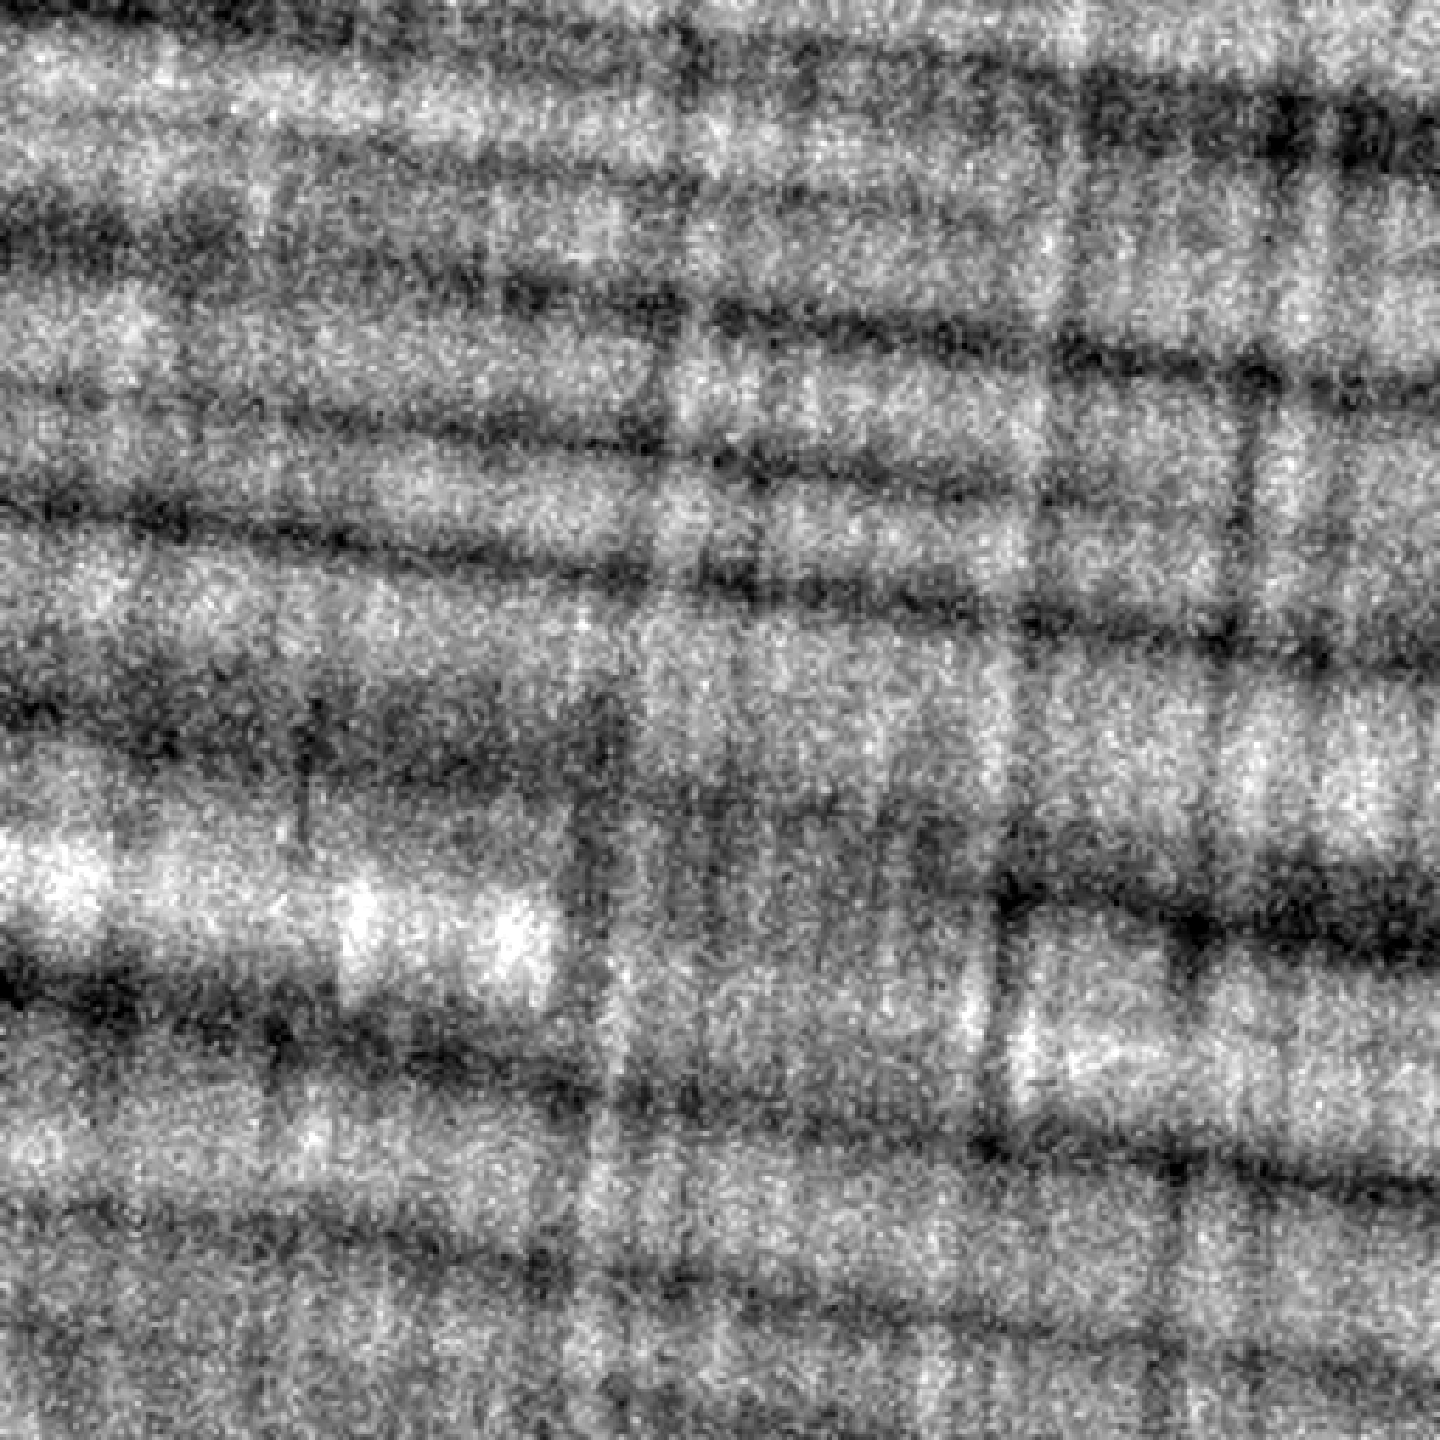
\includegraphics[width=\linewidth]{JS716_20X20.png}
        \caption{JS716}
        \label{fig:a}
    \end{subfigure}
    \hfill
    \begin{subfigure}{0.3\textwidth}
        \centering
        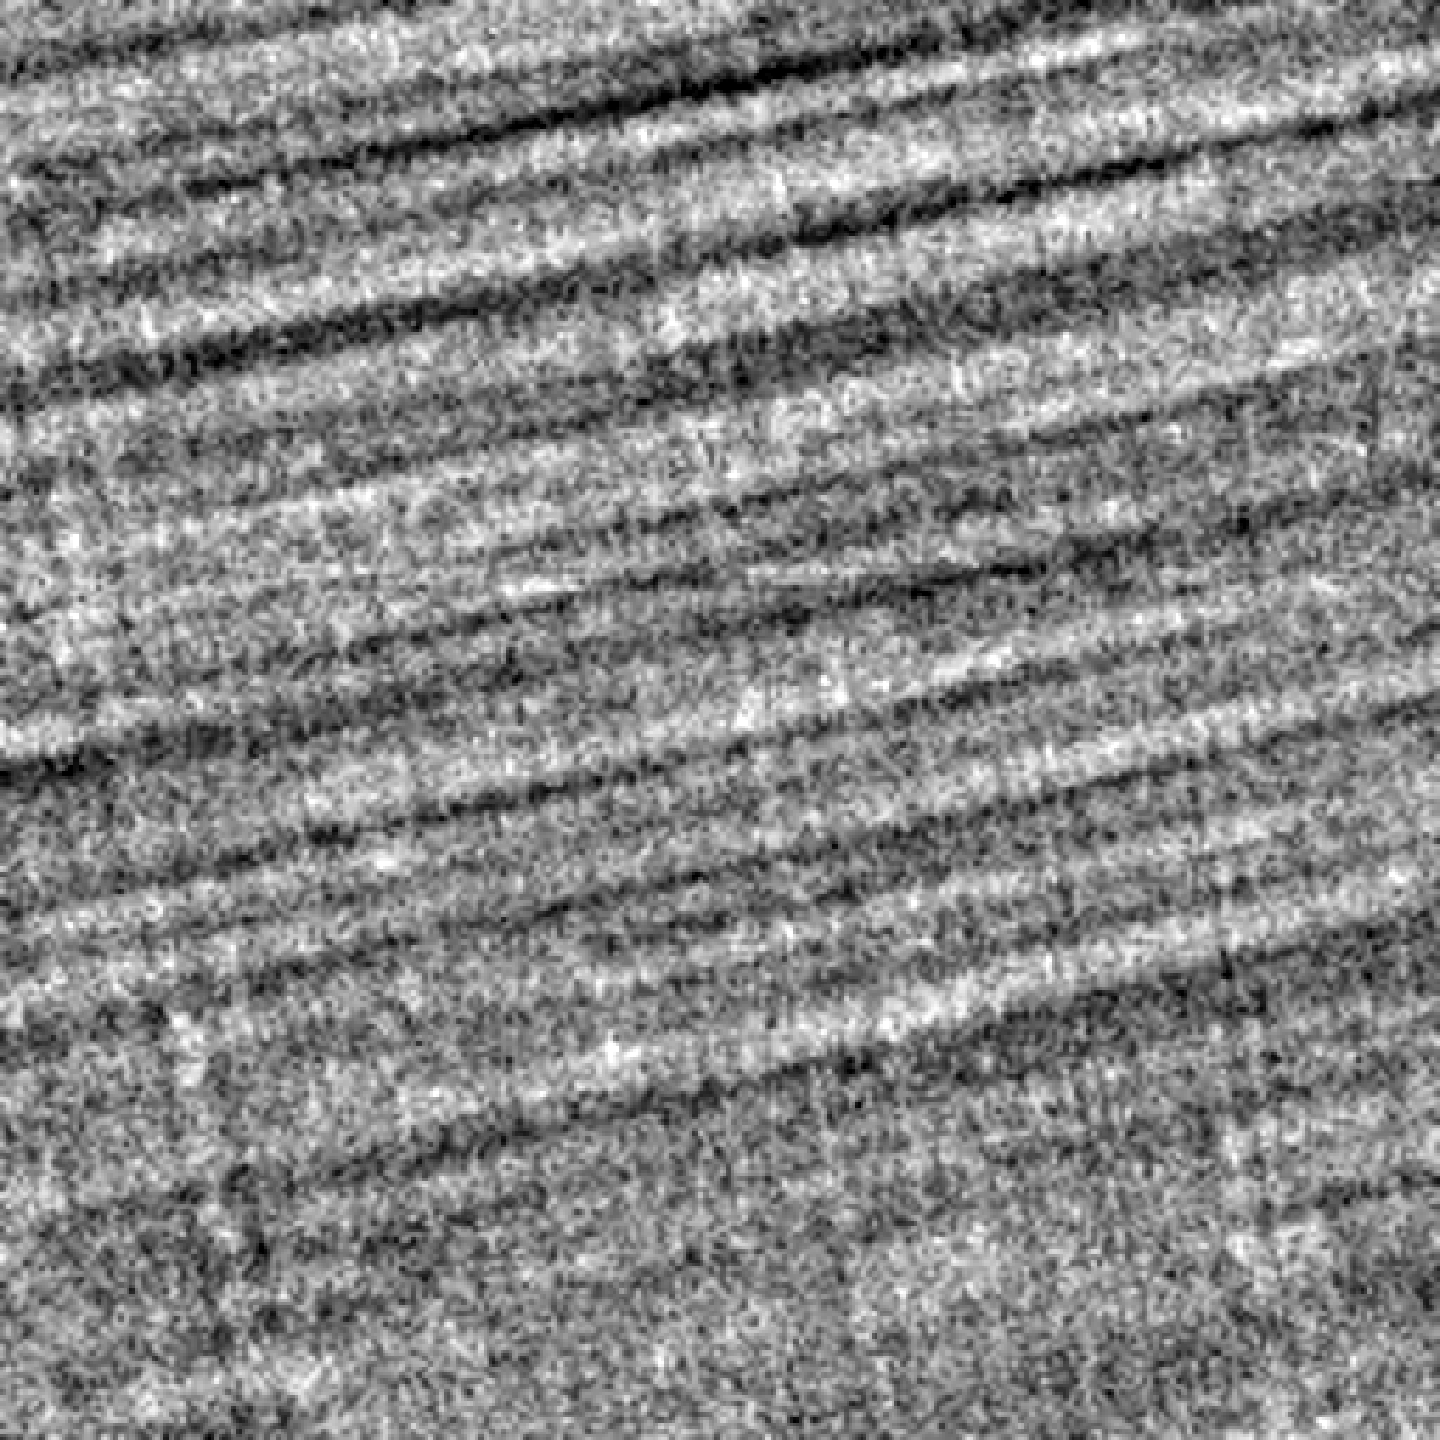
\includegraphics[width=\linewidth]{JS719_20X20.png}
        \caption{JS719}
        \label{fig:b}
    \end{subfigure}
    \hfill
    \begin{subfigure}{0.3\textwidth}
        \centering
        \includegraphics[width=\linewidth]{JS777_20x20.png}
        \caption{JS777}
        \label{fig:c}
    \end{subfigure}
    
    \caption{20$\mu$mx20$\mu$m AFM images of 3 samples, S716 has a mean free path of of 332nm, JS719 has a mean free path of 239nm. The afm image of JS777 shows shows distortions from tip drift and other artifacts.}
    \label{fig:main}
\end{figure}

\bibliographystyle{unsrt}
\bibliography{references}
\end{document}

